\documentclass[1p]{elsarticle_modified}
%\bibliographystyle{elsarticle-num}

%\usepackage[colorlinks]{hyperref}
%\usepackage{abbrmath_seonhwa} %\Abb, \Ascr, \Acal ,\Abf, \Afrak
\usepackage{amsfonts}
\usepackage{amssymb}
\usepackage{amsmath}
\usepackage{amsthm}
\usepackage{scalefnt}
\usepackage{amsbsy}
\usepackage{kotex}
\usepackage{caption}
\usepackage{subfig}
\usepackage{color}
\usepackage{graphicx}
\usepackage{xcolor} %% white, black, red, green, blue, cyan, magenta, yellow
\usepackage{float}
\usepackage{setspace}
\usepackage{hyperref}

\usepackage{tikz}
\usetikzlibrary{arrows}

\usepackage{multirow}
\usepackage{array} % fixed length table
\usepackage{hhline}

%%%%%%%%%%%%%%%%%%%%%
\makeatletter
\renewcommand*\env@matrix[1][\arraystretch]{%
	\edef\arraystretch{#1}%
	\hskip -\arraycolsep
	\let\@ifnextchar\new@ifnextchar
	\array{*\c@MaxMatrixCols c}}
\makeatother %https://tex.stackexchange.com/questions/14071/how-can-i-increase-the-line-spacing-in-a-matrix
%%%%%%%%%%%%%%%

\usepackage[normalem]{ulem}

\newcommand{\msout}[1]{\ifmmode\text{\sout{\ensuremath{#1}}}\else\sout{#1}\fi}
%SOURCE: \msout is \stkout macro in https://tex.stackexchange.com/questions/20609/strikeout-in-math-mode

\newcommand{\cancel}[1]{
	\ifmmode
	{\color{red}\msout{#1}}
	\else
	{\color{red}\sout{#1}}
	\fi
}

\newcommand{\add}[1]{
	{\color{blue}\uwave{#1}}
}

\newcommand{\replace}[2]{
	\ifmmode
	{\color{red}\msout{#1}}{\color{blue}\uwave{#2}}
	\else
	{\color{red}\sout{#1}}{\color{blue}\uwave{#2}}
	\fi
}

\newcommand{\Sol}{\mathcal{S}} %segment
\newcommand{\D}{D} %diagram
\newcommand{\A}{\mathcal{A}} %arc


%%%%%%%%%%%%%%%%%%%%%%%%%%%%%5 test

\def\sl{\operatorname{\textup{SL}}(2,\Cbb)}
\def\psl{\operatorname{\textup{PSL}}(2,\Cbb)}
\def\quan{\mkern 1mu \triangleright \mkern 1mu}

\theoremstyle{definition}
\newtheorem{thm}{Theorem}[section]
\newtheorem{prop}[thm]{Proposition}
\newtheorem{lem}[thm]{Lemma}
\newtheorem{ques}[thm]{Question}
\newtheorem{cor}[thm]{Corollary}
\newtheorem{defn}[thm]{Definition}
\newtheorem{exam}[thm]{Example}
\newtheorem{rmk}[thm]{Remark}
\newtheorem{alg}[thm]{Algorithm}

\newcommand{\I}{\sqrt{-1}}
\begin{document}

%\begin{frontmatter}
%
%\title{Boundary parabolic representations of knots up to 8 crossings}
%
%%% Group authors per affiliation:
%\author{Yunhi Cho} 
%\address{Department of Mathematics, University of Seoul, Seoul, Korea}
%\ead{yhcho@uos.ac.kr}
%
%
%\author{Seonhwa Kim} %\fnref{s_kim}}
%\address{Center for Geometry and Physics, Institute for Basic Science, Pohang, 37673, Korea}
%\ead{ryeona17@ibs.re.kr}
%
%\author{Hyuk Kim}
%\address{Department of Mathematical Sciences, Seoul National University, Seoul 08826, Korea}
%\ead{hyukkim@snu.ac.kr}
%
%\author{Seokbeom Yoon}
%\address{Department of Mathematical Sciences, Seoul National University, Seoul, 08826,  Korea}
%\ead{sbyoon15@snu.ac.kr}
%
%\begin{abstract}
%We find all boundary parabolic representation of knots up to 8 crossings.
%
%\end{abstract}
%\begin{keyword}
%    \MSC[2010] 57M25 
%\end{keyword}
%
%\end{frontmatter}

%\linenumbers
%\tableofcontents
%
\newcommand\colored[1]{\textcolor{white}{\rule[-0.35ex]{0.8em}{1.4ex}}\kern-0.8em\color{red} #1}%
%\newcommand\colored[1]{\textcolor{white}{ #1}\kern-2.17ex	\textcolor{white}{ #1}\kern-1.81ex	\textcolor{white}{ #1}\kern-2.15ex\color{red}#1	}

{\Large $\underline{11a_{20}~(K11a_{20})}$}

\setlength{\tabcolsep}{10pt}
\renewcommand{\arraystretch}{1.6}
\vspace{1cm}\begin{tabular}{m{100pt}>{\centering\arraybackslash}m{274pt}}
\multirow{5}{120pt}{
	\centering
	\includegraphics[width=112pt]{../../../GIT/diagram.site/Diagrams/png/269_11a_20.png}\\
\ \ \ A knot diagram\footnotemark}&
\allowdisplaybreaks
\textbf{Linearized knot diagam} \\
\cline{2-2}
 &
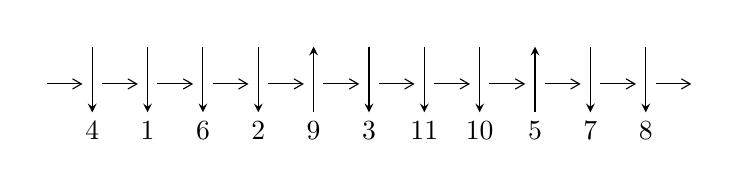
\begin{tikzpicture}[x=20pt, y=17pt]
	% nodes
	\node (C0) at (0, 0) {};
	\node (C1) at (1, 0) {};
	\node (C1U) at (1, +1) {};
	\node (C1D) at (1, -1) {4};

	\node (C2) at (2, 0) {};
	\node (C2U) at (2, +1) {};
	\node (C2D) at (2, -1) {1};

	\node (C3) at (3, 0) {};
	\node (C3U) at (3, +1) {};
	\node (C3D) at (3, -1) {6};

	\node (C4) at (4, 0) {};
	\node (C4U) at (4, +1) {};
	\node (C4D) at (4, -1) {2};

	\node (C5) at (5, 0) {};
	\node (C5U) at (5, +1) {};
	\node (C5D) at (5, -1) {9};

	\node (C6) at (6, 0) {};
	\node (C6U) at (6, +1) {};
	\node (C6D) at (6, -1) {3};

	\node (C7) at (7, 0) {};
	\node (C7U) at (7, +1) {};
	\node (C7D) at (7, -1) {11};

	\node (C8) at (8, 0) {};
	\node (C8U) at (8, +1) {};
	\node (C8D) at (8, -1) {10};

	\node (C9) at (9, 0) {};
	\node (C9U) at (9, +1) {};
	\node (C9D) at (9, -1) {5};

	\node (C10) at (10, 0) {};
	\node (C10U) at (10, +1) {};
	\node (C10D) at (10, -1) {7};

	\node (C11) at (11, 0) {};
	\node (C11U) at (11, +1) {};
	\node (C11D) at (11, -1) {8};
	\node (C12) at (12, 0) {};

	% arrows
	\draw[->,>={angle 60}]
	(C0) edge (C1) (C1) edge (C2) (C2) edge (C3) (C3) edge (C4) (C4) edge (C5) (C5) edge (C6) (C6) edge (C7) (C7) edge (C8) (C8) edge (C9) (C9) edge (C10) (C10) edge (C11) (C11) edge (C12) ;	\draw[->,>=stealth]
	(C1U) edge (C1D) (C2U) edge (C2D) (C3U) edge (C3D) (C4U) edge (C4D) (C5D) edge (C5U) (C6U) edge (C6D) (C7U) edge (C7D) (C8U) edge (C8D) (C9D) edge (C9U) (C10U) edge (C10D) (C11U) edge (C11D) ;
	\end{tikzpicture} \\
\hhline{~~} \\& 
\textbf{Solving Sequence} \\ \cline{2-2} 
 &
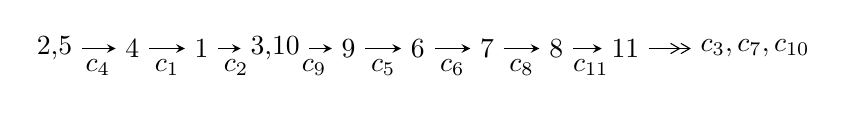
\begin{tikzpicture}[x=25pt, y=7pt]
	% node
	\node (A0) at (-1/8, 0) {2,5};
	\node (A1) at (1, 0) {4};
	\node (A2) at (2, 0) {1};
	\node (A3) at (49/16, 0) {3,10};
	\node (A4) at (33/8, 0) {9};
	\node (A5) at (41/8, 0) {6};
	\node (A6) at (49/8, 0) {7};
	\node (A7) at (57/8, 0) {8};
	\node (A8) at (65/8, 0) {11};
	\node (C1) at (1/2, -1) {$c_{4}$};
	\node (C2) at (3/2, -1) {$c_{1}$};
	\node (C3) at (5/2, -1) {$c_{2}$};
	\node (C4) at (29/8, -1) {$c_{9}$};
	\node (C5) at (37/8, -1) {$c_{5}$};
	\node (C6) at (45/8, -1) {$c_{6}$};
	\node (C7) at (53/8, -1) {$c_{8}$};
	\node (C8) at (61/8, -1) {$c_{11}$};
	\node (A9) at (10, 0) {$c_{3},c_{7},c_{10}$};

	% edge
	\draw[->,>=stealth]	
	(A0) edge (A1) (A1) edge (A2) (A2) edge (A3) (A3) edge (A4) (A4) edge (A5) (A5) edge (A6) (A6) edge (A7) (A7) edge (A8) ;
	\draw[->>,>={angle 60}]	
	(A8) edge (A9);
\end{tikzpicture} \\ 

\end{tabular} \\

\footnotetext{
The image of knot diagram is generated by the software ``\textbf{Draw programme}" developed by Andrew Bartholomew(\url{http://www.layer8.co.uk/maths/draw/index.htm\#Running-draw}), where we modified some parts for our purpose(\url{https://github.com/CATsTAILs/LinksPainter}).
}\phantom \\ \newline 
\centering \textbf{Ideals for irreducible components\footnotemark of $X_{\text{par}}$} 
 
\begin{align*}
I^u_{1}&=\langle 
-2.27448\times10^{21} u^{63}+1.27056\times10^{22} u^{62}+\cdots+4.69870\times10^{20} b+1.19330\times10^{21},\\
\phantom{I^u_{1}}&\phantom{= \langle  }-5.52423\times10^{21} u^{63}+2.53933\times10^{22} u^{62}+\cdots+9.39740\times10^{20} a+2.28536\times10^{20},\;u^{64}-7 u^{63}+\cdots+u+1\rangle \\
I^u_{2}&=\langle 
- a^4+a^3- a^2+b+2 a-1,\;a^5- a^4+a^3-2 a^2+a-1,\;u+1\rangle \\
I^u_{3}&=\langle 
b,\;u^2+a-2 u+1,\;u^3- u^2+1\rangle \\
\\
\end{align*}
\raggedright * 3 irreducible components of $\dim_{\mathbb{C}}=0$, with total 72 representations.\\
\footnotetext{All coefficients of polynomials are rational numbers. But the coefficients are sometimes approximated in decimal forms when there is not enough margin.}
\newpage
\renewcommand{\arraystretch}{1}
\centering \section*{I. $I^u_{1}= \langle -2.27\times10^{21} u^{63}+1.27\times10^{22} u^{62}+\cdots+4.70\times10^{20} b+1.19\times10^{21},\;-5.52\times10^{21} u^{63}+2.54\times10^{22} u^{62}+\cdots+9.40\times10^{20} a+2.29\times10^{20},\;u^{64}-7 u^{63}+\cdots+u+1 \rangle$}
\flushleft \textbf{(i) Arc colorings}\\
\begin{tabular}{m{7pt} m{180pt} m{7pt} m{180pt} }
\flushright $a_{2}=$&$\begin{pmatrix}0\\u\end{pmatrix}$ \\
\flushright $a_{5}=$&$\begin{pmatrix}1\\0\end{pmatrix}$ \\
\flushright $a_{4}=$&$\begin{pmatrix}1\\- u^2\end{pmatrix}$ \\
\flushright $a_{1}=$&$\begin{pmatrix}u\\- u^3+u\end{pmatrix}$ \\
\flushright $a_{3}=$&$\begin{pmatrix}- u^3\\u^5- u^3+u\end{pmatrix}$ \\
\flushright $a_{10}=$&$\begin{pmatrix}5.87847 u^{63}-27.0216 u^{62}+\cdots+28.2191 u-0.243190\\4.84066 u^{63}-27.0407 u^{62}+\cdots+0.696184 u-2.53964\end{pmatrix}$ \\
\flushright $a_{9}=$&$\begin{pmatrix}1.03781 u^{63}+0.0190663 u^{62}+\cdots+27.5230 u+2.29645\\4.84066 u^{63}-27.0407 u^{62}+\cdots+0.696184 u-2.53964\end{pmatrix}$ \\
\flushright $a_{6}=$&$\begin{pmatrix}10.4449 u^{63}-79.7256 u^{62}+\cdots-50.1840 u-25.9116\\0.631883 u^{63}+8.05715 u^{62}+\cdots+34.0330 u+11.6574\end{pmatrix}$ \\
\flushright $a_{7}=$&$\begin{pmatrix}5.78835 u^{63}-39.8513 u^{62}+\cdots-14.9790 u-11.2988\\-2.02198 u^{63}+22.2471 u^{62}+\cdots+31.7864 u+11.7439\end{pmatrix}$ \\
\flushright $a_{8}=$&$\begin{pmatrix}13.3094 u^{63}-73.2209 u^{62}+\cdots+17.5988 u-8.10092\\-4.44093 u^{63}+37.8664 u^{62}+\cdots+36.2343 u+13.7317\end{pmatrix}$ \\
\flushright $a_{11}=$&$\begin{pmatrix}17.7393 u^{63}-103.819 u^{62}+\cdots+2.17710 u-17.2081\\-2.67789 u^{63}+31.9650 u^{62}+\cdots+50.1233 u+17.4101\end{pmatrix}$\\ \flushright $a_{11}=$&$\begin{pmatrix}17.7393 u^{63}-103.819 u^{62}+\cdots+2.17710 u-17.2081\\-2.67789 u^{63}+31.9650 u^{62}+\cdots+50.1233 u+17.4101\end{pmatrix}$\\&\end{tabular}
\flushleft \textbf{(ii) Obstruction class $= -1$}\\~\\
\flushleft \textbf{(iii) Cusp Shapes $= \frac{2720935457231122035033}{469870013462984070152} u^{63}-\frac{8461485863841657548067}{469870013462984070152} u^{62}+\cdots+\frac{14151995465501805816563}{469870013462984070152} u+\frac{1148701840102396678745}{117467503365746017538}$}\\~\\
\newpage\renewcommand{\arraystretch}{1}
\flushleft \textbf{(iv) u-Polynomials at the component}\newline \\
\begin{tabular}{m{50pt}|m{274pt}}
Crossings & \hspace{64pt}u-Polynomials at each crossing \\
\hline $$\begin{aligned}c_{1},c_{4}\end{aligned}$$&$\begin{aligned}
&u^{64}-7 u^{63}+\cdots+u+1
\end{aligned}$\\
\hline $$\begin{aligned}c_{2}\end{aligned}$$&$\begin{aligned}
&u^{64}+29 u^{63}+\cdots+27 u+1
\end{aligned}$\\
\hline $$\begin{aligned}c_{3},c_{6}\end{aligned}$$&$\begin{aligned}
&u^{64}-2 u^{63}+\cdots+64 u-32
\end{aligned}$\\
\hline $$\begin{aligned}c_{5},c_{9}\end{aligned}$$&$\begin{aligned}
&u^{64}-2 u^{63}+\cdots+4 u+8
\end{aligned}$\\
\hline $$\begin{aligned}c_{7},c_{10},c_{11}\end{aligned}$$&$\begin{aligned}
&u^{64}-5 u^{63}+\cdots+14 u-1
\end{aligned}$\\
\hline $$\begin{aligned}c_{8}\end{aligned}$$&$\begin{aligned}
&u^{64}+24 u^{63}+\cdots-464 u+64
\end{aligned}$\\
\hline
\end{tabular}\\~\\
\newpage\renewcommand{\arraystretch}{1}
\flushleft \textbf{(v) Riley Polynomials at the component}\newline \\
\begin{tabular}{m{50pt}|m{274pt}}
Crossings & \hspace{64pt}Riley Polynomials at each crossing \\
\hline $$\begin{aligned}c_{1},c_{4}\end{aligned}$$&$\begin{aligned}
&y^{64}-29 y^{63}+\cdots-27 y+1
\end{aligned}$\\
\hline $$\begin{aligned}c_{2}\end{aligned}$$&$\begin{aligned}
&y^{64}+19 y^{63}+\cdots-2587 y+1
\end{aligned}$\\
\hline $$\begin{aligned}c_{3},c_{6}\end{aligned}$$&$\begin{aligned}
&y^{64}+36 y^{63}+\cdots+7680 y+1024
\end{aligned}$\\
\hline $$\begin{aligned}c_{5},c_{9}\end{aligned}$$&$\begin{aligned}
&y^{64}+24 y^{63}+\cdots-464 y+64
\end{aligned}$\\
\hline $$\begin{aligned}c_{7},c_{10},c_{11}\end{aligned}$$&$\begin{aligned}
&y^{64}-55 y^{63}+\cdots-294 y+1
\end{aligned}$\\
\hline $$\begin{aligned}c_{8}\end{aligned}$$&$\begin{aligned}
&y^{64}+28 y^{63}+\cdots-1248512 y+4096
\end{aligned}$\\
\hline
\end{tabular}\\~\\
\newpage\flushleft \textbf{(vi) Complex Volumes and Cusp Shapes}
$$\begin{array}{c|c|c}  
\text{Solutions to }I^u_{1}& \I (\text{vol} + \sqrt{-1}CS) & \text{Cusp shape}\\
 \hline 
\begin{aligned}
u &= \phantom{-}0.892738 + 0.448763 I \\
a &= -0.677948 - 0.577752 I \\
b &= -1.105160 + 0.138131 I\end{aligned}
 & -3.21351 - 1.80870 I & \phantom{-0.000000 } 0 \\ \hline\begin{aligned}
u &= \phantom{-}0.892738 - 0.448763 I \\
a &= -0.677948 + 0.577752 I \\
b &= -1.105160 - 0.138131 I\end{aligned}
 & -3.21351 + 1.80870 I & \phantom{-0.000000 } 0 \\ \hline\begin{aligned}
u &= \phantom{-}0.455631 + 0.904878 I \\
a &= -1.188140 - 0.429481 I \\
b &= -0.722344 - 0.983370 I\end{aligned}
 & \phantom{-}5.23941 + 5.04408 I & \phantom{-0.000000 } 0 \\ \hline\begin{aligned}
u &= \phantom{-}0.455631 - 0.904878 I \\
a &= -1.188140 + 0.429481 I \\
b &= -0.722344 + 0.983370 I\end{aligned}
 & \phantom{-}5.23941 - 5.04408 I & \phantom{-0.000000 } 0 \\ \hline\begin{aligned}
u &= \phantom{-}0.458581 + 0.849452 I \\
a &= \phantom{-}1.68790 - 0.08561 I \\
b &= \phantom{-}0.950572 - 0.661117 I\end{aligned}
 & \phantom{-}1.85655 + 3.18076 I & -7.00000 + 0. I\phantom{ +0.000000I} \\ \hline\begin{aligned}
u &= \phantom{-}0.458581 - 0.849452 I \\
a &= \phantom{-}1.68790 + 0.08561 I \\
b &= \phantom{-}0.950572 + 0.661117 I\end{aligned}
 & \phantom{-}1.85655 - 3.18076 I & -7.00000 + 0. I\phantom{ +0.000000I} \\ \hline\begin{aligned}
u &= \phantom{-}0.513790 + 0.814105 I \\
a &= \phantom{-}1.137550 + 0.030043 I \\
b &= \phantom{-}0.641399 + 0.876706 I\end{aligned}
 & \phantom{-}2.25186 + 0.42541 I & -7.00000 + 0. I\phantom{ +0.000000I} \\ \hline\begin{aligned}
u &= \phantom{-}0.513790 - 0.814105 I \\
a &= \phantom{-}1.137550 - 0.030043 I \\
b &= \phantom{-}0.641399 - 0.876706 I\end{aligned}
 & \phantom{-}2.25186 - 0.42541 I & -7.00000 + 0. I\phantom{ +0.000000I} \\ \hline\begin{aligned}
u &= \phantom{-}0.575812 + 0.867424 I \\
a &= -1.40928 + 0.24972 I \\
b &= -0.808864 + 0.726024 I\end{aligned}
 & \phantom{-}6.03567 - 0.70423 I & \phantom{-0.000000 } 0 \\ \hline\begin{aligned}
u &= \phantom{-}0.575812 - 0.867424 I \\
a &= -1.40928 - 0.24972 I \\
b &= -0.808864 - 0.726024 I\end{aligned}
 & \phantom{-}6.03567 + 0.70423 I & \phantom{-0.000000 } 0\\
 \hline 
 \end{array}$$\newpage$$\begin{array}{c|c|c}  
\text{Solutions to }I^u_{1}& \I (\text{vol} + \sqrt{-1}CS) & \text{Cusp shape}\\
 \hline 
\begin{aligned}
u &= \phantom{-}0.404010 + 0.961178 I \\
a &= \phantom{-}1.161090 + 0.684160 I \\
b &= \phantom{-}0.751183 + 1.083290 I\end{aligned}
 & \phantom{-}0.50492 + 9.42816 I & \phantom{-0.000000 } 0 \\ \hline\begin{aligned}
u &= \phantom{-}0.404010 - 0.961178 I \\
a &= \phantom{-}1.161090 - 0.684160 I \\
b &= \phantom{-}0.751183 - 1.083290 I\end{aligned}
 & \phantom{-}0.50492 - 9.42816 I & \phantom{-0.000000 } 0 \\ \hline\begin{aligned}
u &= -0.926583 + 0.484056 I \\
a &= -1.11157 + 1.26592 I \\
b &= -0.870442 + 0.528800 I\end{aligned}
 & -2.88218 + 3.00440 I & \phantom{-0.000000 } 0 \\ \hline\begin{aligned}
u &= -0.926583 - 0.484056 I \\
a &= -1.11157 - 1.26592 I \\
b &= -0.870442 - 0.528800 I\end{aligned}
 & -2.88218 - 3.00440 I & \phantom{-0.000000 } 0 \\ \hline\begin{aligned}
u &= -1.043140 + 0.195913 I \\
a &= -0.91468 + 1.70928 I \\
b &= \phantom{-}0.025861 - 0.692002 I\end{aligned}
 & -2.98471 + 0.79780 I & \phantom{-0.000000 } 0 \\ \hline\begin{aligned}
u &= -1.043140 - 0.195913 I \\
a &= -0.91468 - 1.70928 I \\
b &= \phantom{-}0.025861 + 0.692002 I\end{aligned}
 & -2.98471 - 0.79780 I & \phantom{-0.000000 } 0 \\ \hline\begin{aligned}
u &= \phantom{-}0.942735 + 0.500566 I \\
a &= \phantom{-}0.607864 + 1.224530 I \\
b &= \phantom{-}0.012514 - 1.072630 I\end{aligned}
 & -1.51825 - 4.24420 I & \phantom{-0.000000 } 0 \\ \hline\begin{aligned}
u &= \phantom{-}0.942735 - 0.500566 I \\
a &= \phantom{-}0.607864 - 1.224530 I \\
b &= \phantom{-}0.012514 + 1.072630 I\end{aligned}
 & -1.51825 + 4.24420 I & \phantom{-0.000000 } 0 \\ \hline\begin{aligned}
u &= -0.842329 + 0.399836 I \\
a &= -2.62253 + 0.97033 I \\
b &= -0.487811 - 0.667717 I\end{aligned}
 & -2.41667 + 0.68003 I & -10.70240 - 3.97154 I \\ \hline\begin{aligned}
u &= -0.842329 - 0.399836 I \\
a &= -2.62253 - 0.97033 I \\
b &= -0.487811 + 0.667717 I\end{aligned}
 & -2.41667 - 0.68003 I & -10.70240 + 3.97154 I\\
 \hline 
 \end{array}$$\newpage$$\begin{array}{c|c|c}  
\text{Solutions to }I^u_{1}& \I (\text{vol} + \sqrt{-1}CS) & \text{Cusp shape}\\
 \hline 
\begin{aligned}
u &= -0.643524 + 0.662505 I \\
a &= -0.81928 + 1.53795 I \\
b &= -0.573528 + 0.999433 I\end{aligned}
 & -3.53655 - 3.75839 I & -9.90897 + 2.47413 I \\ \hline\begin{aligned}
u &= -0.643524 - 0.662505 I \\
a &= -0.81928 - 1.53795 I \\
b &= -0.573528 - 0.999433 I\end{aligned}
 & -3.53655 + 3.75839 I & -9.90897 - 2.47413 I \\ \hline\begin{aligned}
u &= -0.924487 + 0.552399 I \\
a &= \phantom{-}2.35170 - 0.32648 I \\
b &= \phantom{-}0.638310 + 0.930488 I\end{aligned}
 & \phantom{-}0.23940 + 4.71266 I & \phantom{-0.000000 } 0 \\ \hline\begin{aligned}
u &= -0.924487 - 0.552399 I \\
a &= \phantom{-}2.35170 + 0.32648 I \\
b &= \phantom{-}0.638310 - 0.930488 I\end{aligned}
 & \phantom{-}0.23940 - 4.71266 I & \phantom{-0.000000 } 0 \\ \hline\begin{aligned}
u &= -0.750013 + 0.530556 I \\
a &= \phantom{-}0.92021 - 1.37826 I \\
b &= \phantom{-}0.649111 - 0.745774 I\end{aligned}
 & \phantom{-}0.803950 - 0.315255 I & -4.55635 + 0. I\phantom{ +0.000000I} \\ \hline\begin{aligned}
u &= -0.750013 - 0.530556 I \\
a &= \phantom{-}0.92021 + 1.37826 I \\
b &= \phantom{-}0.649111 + 0.745774 I\end{aligned}
 & \phantom{-}0.803950 + 0.315255 I & -4.55635 + 0. I\phantom{ +0.000000I} \\ \hline\begin{aligned}
u &= \phantom{-}0.813121 + 0.418560 I \\
a &= -0.127255 - 1.035700 I \\
b &= \phantom{-}0.284466 + 1.063420 I\end{aligned}
 & -0.924060 + 0.442031 I & -7.00000 + 0. I\phantom{ +0.000000I} \\ \hline\begin{aligned}
u &= \phantom{-}0.813121 - 0.418560 I \\
a &= -0.127255 + 1.035700 I \\
b &= \phantom{-}0.284466 - 1.063420 I\end{aligned}
 & -0.924060 - 0.442031 I & -7.00000 + 0. I\phantom{ +0.000000I} \\ \hline\begin{aligned}
u &= \phantom{-}0.861442 + 0.662767 I \\
a &= \phantom{-}0.499053 + 0.320374 I \\
b &= \phantom{-}0.602748 - 0.054842 I\end{aligned}
 & \phantom{-}2.28792 - 2.57835 I & \phantom{-0.000000 } 0 \\ \hline\begin{aligned}
u &= \phantom{-}0.861442 - 0.662767 I \\
a &= \phantom{-}0.499053 - 0.320374 I \\
b &= \phantom{-}0.602748 + 0.054842 I\end{aligned}
 & \phantom{-}2.28792 + 2.57835 I & \phantom{-0.000000 } 0\\
 \hline 
 \end{array}$$\newpage$$\begin{array}{c|c|c}  
\text{Solutions to }I^u_{1}& \I (\text{vol} + \sqrt{-1}CS) & \text{Cusp shape}\\
 \hline 
\begin{aligned}
u &= \phantom{-}0.841966 + 0.249603 I \\
a &= \phantom{-}0.106480 + 0.758428 I \\
b &= -0.493505 - 1.278120 I\end{aligned}
 & -7.08020 + 3.75832 I & -7.89460 + 2.35018 I \\ \hline\begin{aligned}
u &= \phantom{-}0.841966 - 0.249603 I \\
a &= \phantom{-}0.106480 - 0.758428 I \\
b &= -0.493505 + 1.278120 I\end{aligned}
 & -7.08020 - 3.75832 I & -7.89460 - 2.35018 I \\ \hline\begin{aligned}
u &= \phantom{-}0.692342 + 0.906468 I \\
a &= \phantom{-}1.135280 - 0.491124 I \\
b &= \phantom{-}0.613430 - 0.823572 I\end{aligned}
 & \phantom{-}2.43022 - 4.49300 I & \phantom{-0.000000 } 0 \\ \hline\begin{aligned}
u &= \phantom{-}0.692342 - 0.906468 I \\
a &= \phantom{-}1.135280 + 0.491124 I \\
b &= \phantom{-}0.613430 + 0.823572 I\end{aligned}
 & \phantom{-}2.43022 + 4.49300 I & \phantom{-0.000000 } 0 \\ \hline\begin{aligned}
u &= -0.988405 + 0.608854 I \\
a &= -2.21838 + 0.08688 I \\
b &= -0.675315 - 1.087940 I\end{aligned}
 & -4.58177 + 8.71812 I & \phantom{-0.000000 } 0 \\ \hline\begin{aligned}
u &= -0.988405 - 0.608854 I \\
a &= -2.21838 - 0.08688 I \\
b &= -0.675315 + 1.087940 I\end{aligned}
 & -4.58177 - 8.71812 I & \phantom{-0.000000 } 0 \\ \hline\begin{aligned}
u &= \phantom{-}1.083340 + 0.462764 I \\
a &= -0.909615 - 0.728843 I \\
b &= -0.220258 + 1.351590 I\end{aligned}
 & -8.76429 - 6.48628 I & \phantom{-0.000000 } 0 \\ \hline\begin{aligned}
u &= \phantom{-}1.083340 - 0.462764 I \\
a &= -0.909615 + 0.728843 I \\
b &= -0.220258 - 1.351590 I\end{aligned}
 & -8.76429 + 6.48628 I & \phantom{-0.000000 } 0 \\ \hline\begin{aligned}
u &= -0.814631\phantom{ +0.000000I} \\
a &= -0.747058\phantom{ +0.000000I} \\
b &= -0.242726\phantom{ +0.000000I}\end{aligned}
 & -1.19032\phantom{ +0.000000I} & -8.27220\phantom{ +0.000000I} \\ \hline\begin{aligned}
u &= -1.188330 + 0.101883 I \\
a &= \phantom{-}0.944463 - 1.011510 I \\
b &= \phantom{-}0.755044 + 0.405276 I\end{aligned}
 & -3.86010 - 0.85522 I & \phantom{-0.000000 } 0\\
 \hline 
 \end{array}$$\newpage$$\begin{array}{c|c|c}  
\text{Solutions to }I^u_{1}& \I (\text{vol} + \sqrt{-1}CS) & \text{Cusp shape}\\
 \hline 
\begin{aligned}
u &= -1.188330 - 0.101883 I \\
a &= \phantom{-}0.944463 + 1.011510 I \\
b &= \phantom{-}0.755044 - 0.405276 I\end{aligned}
 & -3.86010 + 0.85522 I & \phantom{-0.000000 } 0 \\ \hline\begin{aligned}
u &= -1.190870 + 0.376705 I \\
a &= \phantom{-}1.075110 - 0.386024 I \\
b &= \phantom{-}0.047966 + 1.176860 I\end{aligned}
 & -9.32581 + 1.34639 I & \phantom{-0.000000 } 0 \\ \hline\begin{aligned}
u &= -1.190870 - 0.376705 I \\
a &= \phantom{-}1.075110 + 0.386024 I \\
b &= \phantom{-}0.047966 - 1.176860 I\end{aligned}
 & -9.32581 - 1.34639 I & \phantom{-0.000000 } 0 \\ \hline\begin{aligned}
u &= \phantom{-}1.081320 + 0.644153 I \\
a &= \phantom{-}1.66629 + 1.06042 I \\
b &= \phantom{-}0.541565 - 0.991647 I\end{aligned}
 & \phantom{-}0.54026 - 5.89102 I & \phantom{-0.000000 } 0 \\ \hline\begin{aligned}
u &= \phantom{-}1.081320 - 0.644153 I \\
a &= \phantom{-}1.66629 - 1.06042 I \\
b &= \phantom{-}0.541565 + 0.991647 I\end{aligned}
 & \phantom{-}0.54026 + 5.89102 I & \phantom{-0.000000 } 0 \\ \hline\begin{aligned}
u &= \phantom{-}1.062570 + 0.695609 I \\
a &= -0.374719 - 0.834857 I \\
b &= -0.838497 - 0.611622 I\end{aligned}
 & \phantom{-}4.55904 - 5.08051 I & \phantom{-0.000000 } 0 \\ \hline\begin{aligned}
u &= \phantom{-}1.062570 - 0.695609 I \\
a &= -0.374719 + 0.834857 I \\
b &= -0.838497 + 0.611622 I\end{aligned}
 & \phantom{-}4.55904 + 5.08051 I & \phantom{-0.000000 } 0 \\ \hline\begin{aligned}
u &= -1.272150 + 0.077417 I \\
a &= -0.289723 - 0.748311 I \\
b &= -0.589111 + 0.855580 I\end{aligned}
 & -0.94885 - 2.33285 I & \phantom{-0.000000 } 0 \\ \hline\begin{aligned}
u &= -1.272150 - 0.077417 I \\
a &= -0.289723 + 0.748311 I \\
b &= -0.589111 - 0.855580 I\end{aligned}
 & -0.94885 + 2.33285 I & \phantom{-0.000000 } 0 \\ \hline\begin{aligned}
u &= \phantom{-}1.007050 + 0.790636 I \\
a &= \phantom{-}0.061235 + 0.831316 I \\
b &= \phantom{-}0.477046 + 0.732746 I\end{aligned}
 & \phantom{-}1.48618 - 1.70443 I & \phantom{-0.000000 } 0\\
 \hline 
 \end{array}$$\newpage$$\begin{array}{c|c|c}  
\text{Solutions to }I^u_{1}& \I (\text{vol} + \sqrt{-1}CS) & \text{Cusp shape}\\
 \hline 
\begin{aligned}
u &= \phantom{-}1.007050 - 0.790636 I \\
a &= \phantom{-}0.061235 - 0.831316 I \\
b &= \phantom{-}0.477046 - 0.732746 I\end{aligned}
 & \phantom{-}1.48618 + 1.70443 I & \phantom{-0.000000 } 0 \\ \hline\begin{aligned}
u &= \phantom{-}1.114390 + 0.645519 I \\
a &= \phantom{-}0.525778 + 0.875080 I \\
b &= \phantom{-}1.057350 + 0.612780 I\end{aligned}
 & -0.11555 - 8.73931 I & \phantom{-0.000000 } 0 \\ \hline\begin{aligned}
u &= \phantom{-}1.114390 - 0.645519 I \\
a &= \phantom{-}0.525778 - 0.875080 I \\
b &= \phantom{-}1.057350 - 0.612780 I\end{aligned}
 & -0.11555 + 8.73931 I & \phantom{-0.000000 } 0 \\ \hline\begin{aligned}
u &= -0.043869 + 0.693831 I \\
a &= \phantom{-}0.223595 - 1.043440 I \\
b &= -0.179019 - 1.111590 I\end{aligned}
 & -5.83041 + 2.67272 I & -11.08007 - 3.60014 I \\ \hline\begin{aligned}
u &= -0.043869 - 0.693831 I \\
a &= \phantom{-}0.223595 + 1.043440 I \\
b &= -0.179019 + 1.111590 I\end{aligned}
 & -5.83041 - 2.67272 I & -11.08007 + 3.60014 I \\ \hline\begin{aligned}
u &= \phantom{-}1.134300 + 0.665213 I \\
a &= -1.79581 - 0.80258 I \\
b &= -0.694107 + 1.060630 I\end{aligned}
 & \phantom{-}3.18001 - 10.81860 I & \phantom{-0.000000 } 0 \\ \hline\begin{aligned}
u &= \phantom{-}1.134300 - 0.665213 I \\
a &= -1.79581 + 0.80258 I \\
b &= -0.694107 - 1.060630 I\end{aligned}
 & \phantom{-}3.18001 + 10.81860 I & \phantom{-0.000000 } 0 \\ \hline\begin{aligned}
u &= \phantom{-}1.174860 + 0.664654 I \\
a &= \phantom{-}1.79983 + 0.62712 I \\
b &= \phantom{-}0.769782 - 1.149600 I\end{aligned}
 & -1.8513 - 15.3455 I & \phantom{-0.000000 } 0 \\ \hline\begin{aligned}
u &= \phantom{-}1.174860 - 0.664654 I \\
a &= \phantom{-}1.79983 - 0.62712 I \\
b &= \phantom{-}0.769782 + 1.149600 I\end{aligned}
 & -1.8513 + 15.3455 I & \phantom{-0.000000 } 0 \\ \hline\begin{aligned}
u &= -1.344220 + 0.130440 I \\
a &= \phantom{-}0.177278 + 0.405955 I \\
b &= \phantom{-}0.617471 - 1.071230 I\end{aligned}
 & -5.71689 - 6.00573 I & \phantom{-0.000000 } 0\\
 \hline 
 \end{array}$$\newpage$$\begin{array}{c|c|c}  
\text{Solutions to }I^u_{1}& \I (\text{vol} + \sqrt{-1}CS) & \text{Cusp shape}\\
 \hline 
\begin{aligned}
u &= -1.344220 - 0.130440 I \\
a &= \phantom{-}0.177278 - 0.405955 I \\
b &= \phantom{-}0.617471 + 1.071230 I\end{aligned}
 & -5.71689 + 6.00573 I & \phantom{-0.000000 } 0 \\ \hline\begin{aligned}
u &= \phantom{-}0.029039 + 0.244733 I \\
a &= -1.77560 + 0.47939 I \\
b &= \phantom{-}0.227592 + 0.697212 I\end{aligned}
 & -0.369684 + 1.136730 I & -4.87497 - 6.04552 I \\ \hline\begin{aligned}
u &= \phantom{-}0.029039 - 0.244733 I \\
a &= -1.77560 - 0.47939 I \\
b &= \phantom{-}0.227592 - 0.697212 I\end{aligned}
 & -0.369684 - 1.136730 I & -4.87497 + 6.04552 I \\ \hline\begin{aligned}
u &= -0.147593\phantom{ +0.000000I} \\
a &= -6.94526\phantom{ +0.000000I} \\
b &= -0.568177\phantom{ +0.000000I}\end{aligned}
 & -2.17596\phantom{ +0.000000I} & -2.85460\phantom{ +0.000000I}\\
 \hline 
 \end{array}$$\newpage\newpage\renewcommand{\arraystretch}{1}
\centering \section*{II. $I^u_{2}= \langle - a^4+a^3- a^2+b+2 a-1,\;a^5- a^4+a^3-2 a^2+a-1,\;u+1 \rangle$}
\flushleft \textbf{(i) Arc colorings}\\
\begin{tabular}{m{7pt} m{180pt} m{7pt} m{180pt} }
\flushright $a_{2}=$&$\begin{pmatrix}0\\-1\end{pmatrix}$ \\
\flushright $a_{5}=$&$\begin{pmatrix}1\\0\end{pmatrix}$ \\
\flushright $a_{4}=$&$\begin{pmatrix}1\\-1\end{pmatrix}$ \\
\flushright $a_{1}=$&$\begin{pmatrix}-1\\0\end{pmatrix}$ \\
\flushright $a_{3}=$&$\begin{pmatrix}1\\-1\end{pmatrix}$ \\
\flushright $a_{10}=$&$\begin{pmatrix}a\\a^4- a^3+a^2-2 a+1\end{pmatrix}$ \\
\flushright $a_{9}=$&$\begin{pmatrix}- a^4+a^3- a^2+3 a-1\\a^4- a^3+a^2-2 a+1\end{pmatrix}$ \\
\flushright $a_{6}=$&$\begin{pmatrix}a^4- a-1\\- a^4+a+1\end{pmatrix}$ \\
\flushright $a_{7}=$&$\begin{pmatrix}a^4- a-1\\- a^4+a+1\end{pmatrix}$ \\
\flushright $a_{8}=$&$\begin{pmatrix}a\\a^3-1\end{pmatrix}$ \\
\flushright $a_{11}=$&$\begin{pmatrix}a^4- a-1\\- a^3+a^2+2\end{pmatrix}$\\ \flushright $a_{11}=$&$\begin{pmatrix}a^4- a-1\\- a^3+a^2+2\end{pmatrix}$\\&\end{tabular}
\flushleft \textbf{(ii) Obstruction class $= 1$}\\~\\
\flushleft \textbf{(iii) Cusp Shapes $= -5 a^4+5 a^3+7 a-14$}\\~\\
\newpage\renewcommand{\arraystretch}{1}
\flushleft \textbf{(iv) u-Polynomials at the component}\newline \\
\begin{tabular}{m{50pt}|m{274pt}}
Crossings & \hspace{64pt}u-Polynomials at each crossing \\
\hline $$\begin{aligned}c_{1}\end{aligned}$$&$\begin{aligned}
&(u-1)^5
\end{aligned}$\\
\hline $$\begin{aligned}c_{2},c_{4}\end{aligned}$$&$\begin{aligned}
&(u+1)^5
\end{aligned}$\\
\hline $$\begin{aligned}c_{3},c_{6}\end{aligned}$$&$\begin{aligned}
&u^5
\end{aligned}$\\
\hline $$\begin{aligned}c_{5}\end{aligned}$$&$\begin{aligned}
&u^5- u^4+2 u^3- u^2+u-1
\end{aligned}$\\
\hline $$\begin{aligned}c_{7}\end{aligned}$$&$\begin{aligned}
&u^5+u^4-2 u^3- u^2+u-1
\end{aligned}$\\
\hline $$\begin{aligned}c_{8}\end{aligned}$$&$\begin{aligned}
&u^5-3 u^4+4 u^3- u^2- u+1
\end{aligned}$\\
\hline $$\begin{aligned}c_{9}\end{aligned}$$&$\begin{aligned}
&u^5+u^4+2 u^3+u^2+u+1
\end{aligned}$\\
\hline $$\begin{aligned}c_{10},c_{11}\end{aligned}$$&$\begin{aligned}
&u^5- u^4-2 u^3+u^2+u+1
\end{aligned}$\\
\hline
\end{tabular}\\~\\
\newpage\renewcommand{\arraystretch}{1}
\flushleft \textbf{(v) Riley Polynomials at the component}\newline \\
\begin{tabular}{m{50pt}|m{274pt}}
Crossings & \hspace{64pt}Riley Polynomials at each crossing \\
\hline $$\begin{aligned}c_{1},c_{2},c_{4}\end{aligned}$$&$\begin{aligned}
&(y-1)^5
\end{aligned}$\\
\hline $$\begin{aligned}c_{3},c_{6}\end{aligned}$$&$\begin{aligned}
&y^5
\end{aligned}$\\
\hline $$\begin{aligned}c_{5},c_{9}\end{aligned}$$&$\begin{aligned}
&y^5+3 y^4+4 y^3+y^2- y-1
\end{aligned}$\\
\hline $$\begin{aligned}c_{7},c_{10},c_{11}\end{aligned}$$&$\begin{aligned}
&y^5-5 y^4+8 y^3-3 y^2- y-1
\end{aligned}$\\
\hline $$\begin{aligned}c_{8}\end{aligned}$$&$\begin{aligned}
&y^5- y^4+8 y^3-3 y^2+3 y-1
\end{aligned}$\\
\hline
\end{tabular}\\~\\
\newpage\flushleft \textbf{(vi) Complex Volumes and Cusp Shapes}
$$\begin{array}{c|c|c}  
\text{Solutions to }I^u_{2}& \I (\text{vol} + \sqrt{-1}CS) & \text{Cusp shape}\\
 \hline 
\begin{aligned}
u &= -1.00000\phantom{ +0.000000I} \\
a &= -0.428550 + 1.039280 I \\
b &= -0.339110 - 0.822375 I\end{aligned}
 & -1.97403 + 1.53058 I & -10.50099 - 3.45976 I \\ \hline\begin{aligned}
u &= -1.00000\phantom{ +0.000000I} \\
a &= -0.428550 - 1.039280 I \\
b &= -0.339110 + 0.822375 I\end{aligned}
 & -1.97403 - 1.53058 I & -10.50099 + 3.45976 I \\ \hline\begin{aligned}
u &= -1.00000\phantom{ +0.000000I} \\
a &= \phantom{-}0.276511 + 0.728237 I \\
b &= \phantom{-}0.455697 - 1.200150 I\end{aligned}
 & -7.51750 - 4.40083 I & -14.3774 + 5.8297 I \\ \hline\begin{aligned}
u &= -1.00000\phantom{ +0.000000I} \\
a &= \phantom{-}0.276511 - 0.728237 I \\
b &= \phantom{-}0.455697 + 1.200150 I\end{aligned}
 & -7.51750 + 4.40083 I & -14.3774 - 5.8297 I \\ \hline\begin{aligned}
u &= -1.00000\phantom{ +0.000000I} \\
a &= \phantom{-}1.30408\phantom{ +0.000000I} \\
b &= \phantom{-}0.766826\phantom{ +0.000000I}\end{aligned}
 & -4.04602\phantom{ +0.000000I} & -8.24330\phantom{ +0.000000I}\\
 \hline 
 \end{array}$$\newpage\newpage\renewcommand{\arraystretch}{1}
\centering \section*{III. $I^u_{3}= \langle b,\;u^2+a-2 u+1,\;u^3- u^2+1 \rangle$}
\flushleft \textbf{(i) Arc colorings}\\
\begin{tabular}{m{7pt} m{180pt} m{7pt} m{180pt} }
\flushright $a_{2}=$&$\begin{pmatrix}0\\u\end{pmatrix}$ \\
\flushright $a_{5}=$&$\begin{pmatrix}1\\0\end{pmatrix}$ \\
\flushright $a_{4}=$&$\begin{pmatrix}1\\- u^2\end{pmatrix}$ \\
\flushright $a_{1}=$&$\begin{pmatrix}u\\- u^2+u+1\end{pmatrix}$ \\
\flushright $a_{3}=$&$\begin{pmatrix}- u^2+1\\- u^2\end{pmatrix}$ \\
\flushright $a_{10}=$&$\begin{pmatrix}- u^2+2 u-1\\0\end{pmatrix}$ \\
\flushright $a_{9}=$&$\begin{pmatrix}- u^2+2 u-1\\0\end{pmatrix}$ \\
\flushright $a_{6}=$&$\begin{pmatrix}1\\0\end{pmatrix}$ \\
\flushright $a_{7}=$&$\begin{pmatrix}- u\\u^2- u-1\end{pmatrix}$ \\
\flushright $a_{8}=$&$\begin{pmatrix}- u^2+2 u-1\\0\end{pmatrix}$ \\
\flushright $a_{11}=$&$\begin{pmatrix}- u^2+3 u-1\\- u^2+u+1\end{pmatrix}$\\ \flushright $a_{11}=$&$\begin{pmatrix}- u^2+3 u-1\\- u^2+u+1\end{pmatrix}$\\&\end{tabular}
\flushleft \textbf{(ii) Obstruction class $= 1$}\\~\\
\flushleft \textbf{(iii) Cusp Shapes $= - u^2+8 u-16$}\\~\\
\newpage\renewcommand{\arraystretch}{1}
\flushleft \textbf{(iv) u-Polynomials at the component}\newline \\
\begin{tabular}{m{50pt}|m{274pt}}
Crossings & \hspace{64pt}u-Polynomials at each crossing \\
\hline $$\begin{aligned}c_{1}\end{aligned}$$&$\begin{aligned}
&u^3+u^2-1
\end{aligned}$\\
\hline $$\begin{aligned}c_{2},c_{6}\end{aligned}$$&$\begin{aligned}
&u^3+u^2+2 u+1
\end{aligned}$\\
\hline $$\begin{aligned}c_{3}\end{aligned}$$&$\begin{aligned}
&u^3- u^2+2 u-1
\end{aligned}$\\
\hline $$\begin{aligned}c_{4}\end{aligned}$$&$\begin{aligned}
&u^3- u^2+1
\end{aligned}$\\
\hline $$\begin{aligned}c_{5},c_{8},c_{9}\end{aligned}$$&$\begin{aligned}
&u^3
\end{aligned}$\\
\hline $$\begin{aligned}c_{7}\end{aligned}$$&$\begin{aligned}
&(u-1)^3
\end{aligned}$\\
\hline $$\begin{aligned}c_{10},c_{11}\end{aligned}$$&$\begin{aligned}
&(u+1)^3
\end{aligned}$\\
\hline
\end{tabular}\\~\\
\newpage\renewcommand{\arraystretch}{1}
\flushleft \textbf{(v) Riley Polynomials at the component}\newline \\
\begin{tabular}{m{50pt}|m{274pt}}
Crossings & \hspace{64pt}Riley Polynomials at each crossing \\
\hline $$\begin{aligned}c_{1},c_{4}\end{aligned}$$&$\begin{aligned}
&y^3- y^2+2 y-1
\end{aligned}$\\
\hline $$\begin{aligned}c_{2},c_{3},c_{6}\end{aligned}$$&$\begin{aligned}
&y^3+3 y^2+2 y-1
\end{aligned}$\\
\hline $$\begin{aligned}c_{5},c_{8},c_{9}\end{aligned}$$&$\begin{aligned}
&y^3
\end{aligned}$\\
\hline $$\begin{aligned}c_{7},c_{10},c_{11}\end{aligned}$$&$\begin{aligned}
&(y-1)^3
\end{aligned}$\\
\hline
\end{tabular}\\~\\
\newpage\flushleft \textbf{(vi) Complex Volumes and Cusp Shapes}
$$\begin{array}{c|c|c}  
\text{Solutions to }I^u_{3}& \I (\text{vol} + \sqrt{-1}CS) & \text{Cusp shape}\\
 \hline 
\begin{aligned}
u &= \phantom{-}0.877439 + 0.744862 I \\
a &= \phantom{-}0.539798 + 0.182582 I \\
b &= \phantom{-0.000000 } 0\end{aligned}
 & \phantom{-}1.37919 - 2.82812 I & -9.19557 + 4.65175 I \\ \hline\begin{aligned}
u &= \phantom{-}0.877439 - 0.744862 I \\
a &= \phantom{-}0.539798 - 0.182582 I \\
b &= \phantom{-0.000000 } 0\end{aligned}
 & \phantom{-}1.37919 + 2.82812 I & -9.19557 - 4.65175 I \\ \hline\begin{aligned}
u &= -0.754878\phantom{ +0.000000I} \\
a &= -3.07960\phantom{ +0.000000I} \\
b &= \phantom{-0.000000 } 0\end{aligned}
 & -2.75839\phantom{ +0.000000I} & -22.6090\phantom{ +0.000000I}\\
 \hline 
 \end{array}$$\newpage
\newpage\renewcommand{\arraystretch}{1}
\centering \section*{ IV. u-Polynomials}
\begin{tabular}{m{50pt}|m{274pt}}
Crossings & \hspace{64pt}u-Polynomials at each crossing \\
\hline $$\begin{aligned}c_{1}\end{aligned}$$&$\begin{aligned}
&((u-1)^5)(u^3+u^2-1)(u^{64}-7 u^{63}+\cdots+u+1)
\end{aligned}$\\
\hline $$\begin{aligned}c_{2}\end{aligned}$$&$\begin{aligned}
&((u+1)^5)(u^3+u^2+2 u+1)(u^{64}+29 u^{63}+\cdots+27 u+1)
\end{aligned}$\\
\hline $$\begin{aligned}c_{3}\end{aligned}$$&$\begin{aligned}
&u^5(u^3- u^2+2 u-1)(u^{64}-2 u^{63}+\cdots+64 u-32)
\end{aligned}$\\
\hline $$\begin{aligned}c_{4}\end{aligned}$$&$\begin{aligned}
&((u+1)^5)(u^3- u^2+1)(u^{64}-7 u^{63}+\cdots+u+1)
\end{aligned}$\\
\hline $$\begin{aligned}c_{5}\end{aligned}$$&$\begin{aligned}
&u^3(u^5- u^4+\cdots+u-1)(u^{64}-2 u^{63}+\cdots+4 u+8)
\end{aligned}$\\
\hline $$\begin{aligned}c_{6}\end{aligned}$$&$\begin{aligned}
&u^5(u^3+u^2+2 u+1)(u^{64}-2 u^{63}+\cdots+64 u-32)
\end{aligned}$\\
\hline $$\begin{aligned}c_{7}\end{aligned}$$&$\begin{aligned}
&((u-1)^3)(u^5+u^4+\cdots+u-1)(u^{64}-5 u^{63}+\cdots+14 u-1)
\end{aligned}$\\
\hline $$\begin{aligned}c_{8}\end{aligned}$$&$\begin{aligned}
&u^3(u^5-3 u^4+\cdots- u+1)(u^{64}+24 u^{63}+\cdots-464 u+64)
\end{aligned}$\\
\hline $$\begin{aligned}c_{9}\end{aligned}$$&$\begin{aligned}
&u^3(u^5+u^4+\cdots+u+1)(u^{64}-2 u^{63}+\cdots+4 u+8)
\end{aligned}$\\
\hline $$\begin{aligned}c_{10},c_{11}\end{aligned}$$&$\begin{aligned}
&((u+1)^3)(u^5- u^4+\cdots+u+1)(u^{64}-5 u^{63}+\cdots+14 u-1)
\end{aligned}$\\
\hline
\end{tabular}\newpage\renewcommand{\arraystretch}{1}
\centering \section*{ V. Riley Polynomials}
\begin{tabular}{m{50pt}|m{274pt}}
Crossings & \hspace{64pt}Riley Polynomials at each crossing \\
\hline $$\begin{aligned}c_{1},c_{4}\end{aligned}$$&$\begin{aligned}
&((y-1)^5)(y^3- y^2+2 y-1)(y^{64}-29 y^{63}+\cdots-27 y+1)
\end{aligned}$\\
\hline $$\begin{aligned}c_{2}\end{aligned}$$&$\begin{aligned}
&((y-1)^5)(y^3+3 y^2+2 y-1)(y^{64}+19 y^{63}+\cdots-2587 y+1)
\end{aligned}$\\
\hline $$\begin{aligned}c_{3},c_{6}\end{aligned}$$&$\begin{aligned}
&y^5(y^3+3 y^2+2 y-1)(y^{64}+36 y^{63}+\cdots+7680 y+1024)
\end{aligned}$\\
\hline $$\begin{aligned}c_{5},c_{9}\end{aligned}$$&$\begin{aligned}
&y^3(y^5+3 y^4+\cdots- y-1)(y^{64}+24 y^{63}+\cdots-464 y+64)
\end{aligned}$\\
\hline $$\begin{aligned}c_{7},c_{10},c_{11}\end{aligned}$$&$\begin{aligned}
&((y-1)^3)(y^5-5 y^4+\cdots- y-1)(y^{64}-55 y^{63}+\cdots-294 y+1)
\end{aligned}$\\
\hline $$\begin{aligned}c_{8}\end{aligned}$$&$\begin{aligned}
&y^3(y^5- y^4+\cdots+3 y-1)(y^{64}+28 y^{63}+\cdots-1248512 y+4096)
\end{aligned}$\\
\hline
\end{tabular}
\vskip 2pc
\end{document}